%% LaTeX template for BSc Computing for Games final year project dissertations
%% by Edward Powley
%% Games Academy, Falmouth University, UK

%% Based on:
%% bare_jrnl.tex
%% V1.4b
%% 2015/08/26
%% by Michael Shell
%% see http://www.michaelshell.org/
%% for current contact information.
%%
%% This is a skeleton file demonstrating the use of IEEEtran.cls
%% (requires IEEEtran.cls version 1.8b or later) with an IEEE
%% journal paper.
%%
%% Support sites:
%% http://www.michaelshell.org/tex/ieeetran/
%% http://www.ctan.org/pkg/ieeetran
%% and
%% http://www.ieee.org/

%%*************************************************************************
%% Legal Notice:
%% This code is offered as-is without any warranty either expressed or
%% implied; without even the implied warranty of MERCHANTABILITY or
%% FITNESS FOR A PARTICULAR PURPOSE! 
%% User assumes all risk.
%% In no event shall the IEEE or any contributor to this code be liable for
%% any damages or losses, including, but not limited to, incidental,
%% consequential, or any other damages, resulting from the use or misuse
%% of any information contained here.
%%
%% All comments are the opinions of their respective authors and are not
%% necessarily endorsed by the IEEE.
%%
%% This work is distributed under the LaTeX Project Public License (LPPL)
%% ( http://www.latex-project.org/ ) version 1.3, and may be freely used,
%% distributed and modified. A copy of the LPPL, version 1.3, is included
%% in the base LaTeX documentation of all distributions of LaTeX released
%% 2003/12/01 or later.
%% Retain all contribution notices and credits.
%% ** Modified files should be clearly indicated as such, including  **
%% ** renaming them and changing author support contact information. **
%%*************************************************************************


\documentclass[journal]{IEEEtran}

\usepackage{graphicx}
% Insert additional usepackage commands here
\usepackage{amsmath}
\usepackage{wrapfig}
\usepackage{todonotes}
\graphicspath{ {./images/} }


\begin{document}
%
% paper title
% Titles are generally capitalized except for words such as a, an, and, as,
% at, but, by, for, in, nor, of, on, or, the, to and up, which are usually
% not capitalized unless they are the first or last word of the title.
% Linebreaks \\ can be used within to get better formatting as desired.
% Do not put math or special symbols in the title.
\title{Comparing Game Tree Search Techniques for General Video Game Artificial Intelligence}
%
%
% author name
%\author{Alastair Rayner - 1507516}
\author{\IEEEauthorblockN{Alastair Rayner\\}
\IEEEauthorblockA{Falmouth Games Academy\\
Falmouth, UK\\
Student ID: 1507516\\
Email: AR185160@falmouth.ac.uk\\}
}

% The paper headers -- please do not change these, but uncomment one of them as appropriate
% Uncomment this one for COMP320
\markboth{COMP320: Research Review and Proposal}{COMP320: Research Review and Proposal}
% Uncomment this one for COMP360
% \markboth{COMP360: Dissertation}{COMP360: Dissertation}

% make the title area
\maketitle

% As a general rule, do not put math, special symbols or citations
% in the abstract or keywords.
\begin{abstract}
	Video games have been used for benchmarking Artificial intelligence techniques, however in many cases the AI use very domain specific knowledge to improve their results. 
	The General Video Game AI (GVG-AI) competition aims to address the issue of creating an Artificial General Intelligence (AGI) which in this context means to create an AI that is able to complete video games albeit not up to a human skill level. The games within the GVG-AI competition are all arcade style game, such as \textit{Pac-Man} and \textit{Zelda}. 
	This paper describes the goals of GVG-AI as well as its rules and challenges, it also covers the different types of tree search techniques used in General Game Playing (GGP) as well as other game search techniques for AGI.
	
\end{abstract}

\section{Introduction}
	\IEEEPARstart{T}{his} paper will compare the tree search techniques used in the General Video Game Artificial Intelligence (GVG-AI) competition.  
	Games play an important role in the development and bench-marking of Artificial Intelligence (AI). This literature review will cover the existing work around the GVG-AI competition and the different solutions that are available.
	The GVG-AI competition is a recurring video game playing competition designed to simulate and benchmark general artificial intelligence. For an AI agent to be tested, they are submitted to the competition site, then they are tested against previously unseen arcade-style video games like the ones shown in figure \ref{fig:VGDL}. The games that the agents are tested against change every year to stop them from becoming too domain specific.

	There is a large amount of tree search techniques used within the GVG-AI competition, many of them are based around Monte Carlo Tree Search (MCTS).This project will compare the success rates of each of the different methods, as well as an in depth comparison as to where each tree search technique succeeds in a set of existing games.

\begin{figure}[h]
		    \centering
		    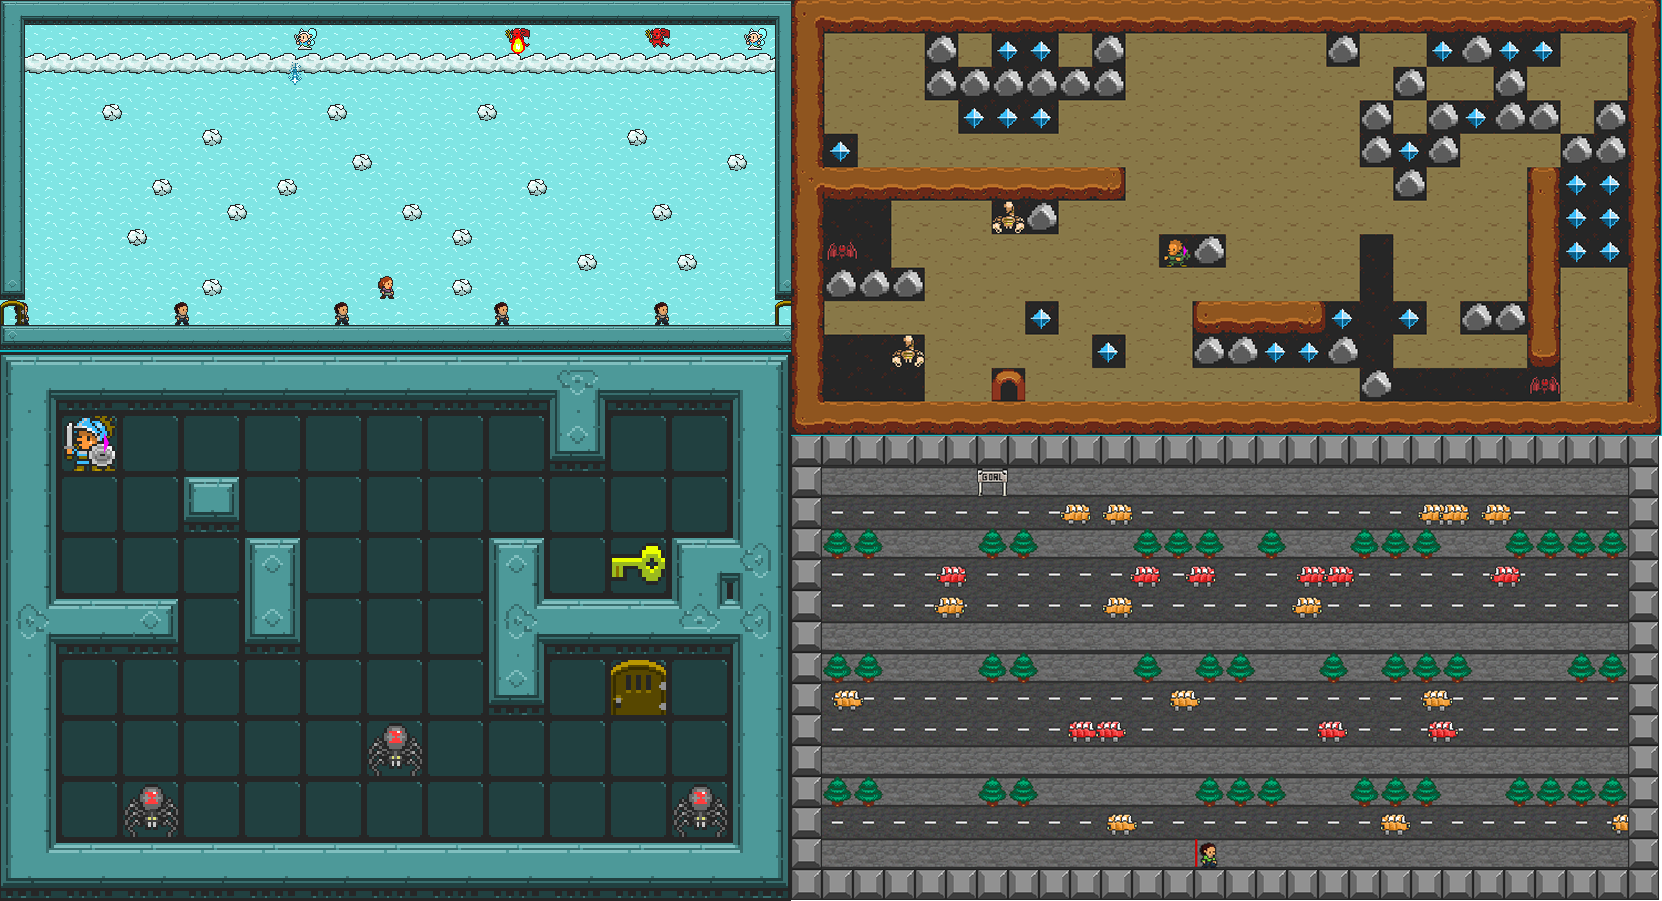
\includegraphics[width=0.5\textwidth]{VGDL2}
		    \caption{Example of games in GVG-AI Framework: angelsdemons (Top Left), boulderdash (Top Right), frogs (Bottom Right), Zelda (Bottom Left). }
		    \label{fig:VGDL}
		\end{figure}
		
\section{Research Questions}

	%Motivation
	There has been considerable literature on GVG-AI and individual AI techniques within the competition, and very little covering an in depth look into the comparison of the different search algorithms.

	Furthermore within the GVG-AI competition there are a few different tree search techniques used, a few of which are mentioned in section \ref{ssec:GST}. 
	These techniques perform quite differently within the competition, this paper will aim to answer \textit{What are the strengths and weaknesses of different search techniques} as well as \textit{What type of game does each search technique succeed at?}


	
	%Importance
	The research gathered from this could lead to a Hyper-Heuristic \footnote{A Hyper-Heuristic contains a portfolio of algorithms and is able to select the most appropriate algorithm to use depending on the game state \cite{hyperHeurisicMendes, horn2016mcts}.}  that can be implemented into a controller for the competition. 
	Furthermore this paper will outline the challenges of using the different search techniques, such as issues of games that have a large search space, or multiple objectives and show what are the most challenging areas for AI within the GVG-AI competition.
	


%What games have too large of a search space for what techniques
%TODO: Simplify research questions
%\begin{itemize}
    %\item How does game tree search techniques compare for GVGAI? 
    %\item Where does each tree search technique do well in each game? 
    %\item What are the strengths and weaknesses of different search techniques and how can they be improved? 
%\end{itemize}


%Does tree search algorithms perform better than Evolutionary Algorithms?
%Where does tree search algorithms out perform Evolutionary Algorithms?

\section{Literature Review}
	\subsection{Artificial General Intelligence in games}
		
		There have been a lot of popular games that have been used to benchmark AI, for example games such as Chess, or Go. Some of these AI programs have been improved upon until they can defeat the world champion players, such as Deep Blue which defeated Garry Kasparov in 1997 \cite{DeepBlue, shannon1988programming, DeepBlueOverview}. 

		%Programming Chess
		Deep Blue was developed at IBM during the mid-1990s. It was able to beat the world chess champion by having a massively parallel system that was able to search a very large search space concurrently \cite{DeepBlue}.

		%Programming Go
		The challenge of creating an AI for the game Go is that it has a huge branching factor and it lacks a good evaluation function (these terms are described in section \ref{sssec:Common}). 
		There have been more recent breakthroughs within AI, such as AlphaGo \cite{silver2016mastering} which was developed by Google Deepmind. It was able to beat the a professional Go player in 2015 and in 2017 was able to beat Ke Jie, the world champion player at the time\cite{silver2016mastering}.
		AlphaGo combined neural networks with MCTS to achieve a 99.8\% win rate against other Go programs. The program used a supervised learning policy network that was trained directly from expert human players, then a reinforcement learning policy network was used to improve the supervised learning policy by optimising the final outcome of self played games. Further information on how this works is described in \cite{silver2016mastering}.
		Monte Carlo Tree Search (MCTS) has had spectacular success in the game Go \cite{browne2012survey}, and is implemented in the top rated go programs.

		During the match against Fan Hui, AlphaGo evaluated thousands of times fewer positions than Deep blue did against Kasparov. It did this by selecting those positions more intelligently using the policy network, then evaluating them more precisely using the value network, where as Deep blue used a more brute force approach \cite{silver2016mastering, DeepBlue}.

		The reason for these AI's success are often as a result of very domain specific knowledge about the game it is playing and means they become highly specialized and cannot be easily ported to other games. 
		This is what started the General Game Playing (GGP) competition (described in section \ref{ssec:GVGAIC}) which was to create general AI for board games, this is similar to what happened with GVG-AI where there was lots of specialized AI for games, which were all very domain specficic, such as Starcraft AI \cite{ontanon2013survey, hingston2010new}.
		This lead to the need for general AI for games, hence GVG-AI and Arcade Learning Environment which is described in section \ref{ssec:GVGAIC}.
		
		A long standing goal of AI is to develop algorithms capable of completing various tasks without any need to create domain specific tailoring.
		
	\subsection{Game Search Techniques} \label{ssec:GST}
		\subsubsection{Common Terms Used in Tree Search Algorithms} \label{sssec:Common}

		\textbf{Branching Factor:}
			Branching Factor is the number of children at each node of a tree. This is a large factor as to what algorithms can be used to play certain types of games, for example; the GVG-AI competition has a maximum branching factor of 7, where as the game Go has a maximum branching factor of 250 \cite{silver2016mastering, perez20162014}.

		\textbf{Horizon Effect:}
			This is the problem where only a small portion of the search tree can be searched, i.e. the AI can search 4 moves ahead, but the 5th move could be a detrimental move, but the AI doesn't know that because its search "\textit{horizon}" is limited \cite{joppen2017informed}.

		\textbf{Evaluation Function:}
			This is used to estimate the value of a position or the current game state, i.e. is the agent winning or loosing the game.
			
		\textbf{Open Loop \& Closed Loop:}
			In the closed loop MCTS the algorithm assumes it is stable to store game sates on the nodes of the tree when expansion is performed, which means that selection can navigate the tree without having to calculate new states.
			In Open Loop MCTS (OLMCTS) the algorithm only stores the statistics on the tree nodes and then generates the next states using the forward model \cite{perez2016analyzing, perez2015open}.
			
		
		
		\subsubsection{Monte Carlo Tree Search (MCTS) }\label{sssec:MCTS}

		Monte Carlo Tree Search is a method for finding the optimal decisions in a specified domain by performing Monte Carlo simulations (taking random samples in the search space and building a search tree according the the results) \cite{browne2012survey}. 

		MCTS is a class of decision tree search algorithms discovered independently by several authors \cite{coulom2006efficient, kocsis2006bandit, chaslot2006monte}.
		
		MCTS has been demonstrated to work effectively with classic board games, modern board-games and video games \cite{chaslot2008monte, pepels2014real}.

		\begin{figure}[h]
		    \centering
		    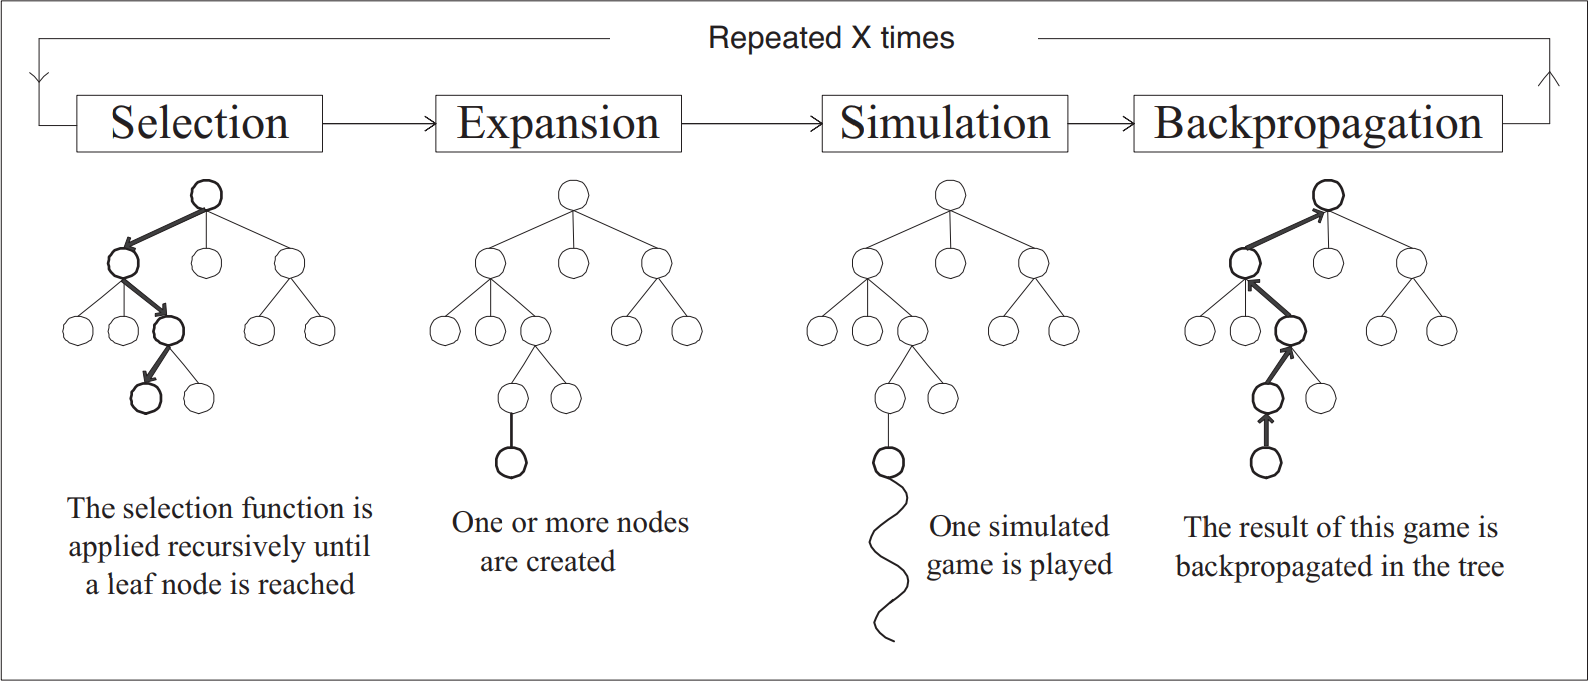
\includegraphics[width=0.5\textwidth]{MCTSProcess}
		    \caption{Overview of Monte Carlo Tree Search. Image sourced from \cite{chaslot2008monte}. }
		    \label{fig:MCTS1}
		\end{figure}
		

		% Explination of MCTS stages
		The basis of MCTS is the simulation of games where both the player controller and the opponent play pseudo-random moves. From playing a single game consisting of random moves, very little can be learnt about the game. However when simulating a multitude of random games, a good strategy can be inferred. This is what MCTS does, it builds a tree of possible future game states. This can described in four stages, as shown in figure \ref{fig:MCTS1}.
				\begin{figure}[h]
		    \centering
		    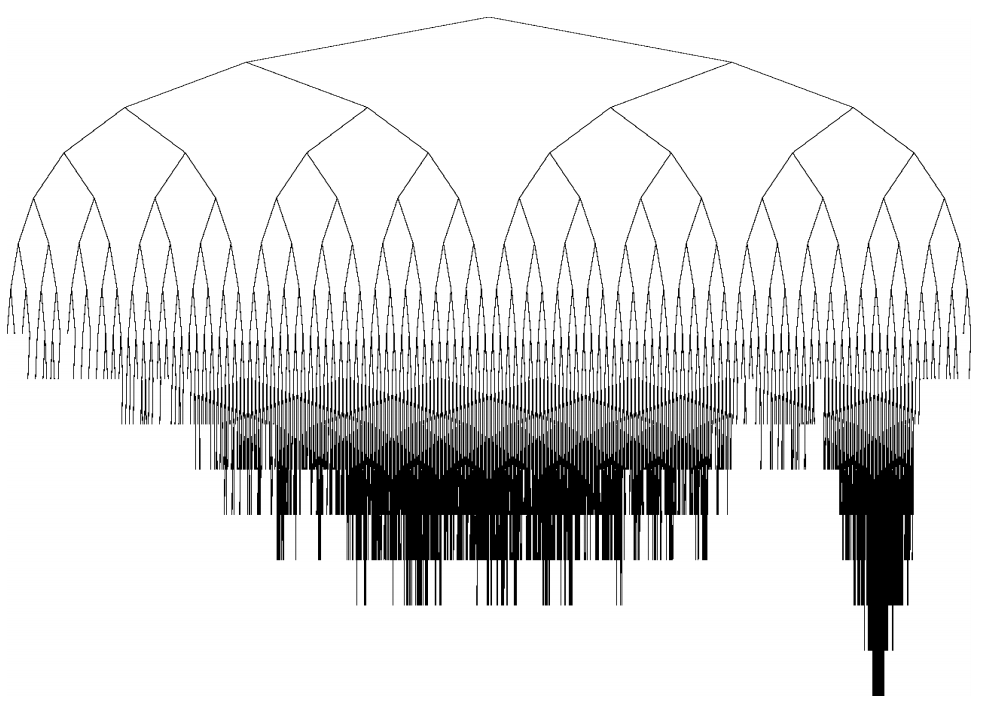
\includegraphics[width=0.5\textwidth]{MCTSasymmetry}
		    \caption{An Example of an Asymmetric Tree Created by MCTS. Image sourced from \cite{coquelin2007bandit}. }
		    \label{fig:MCTS2}
		\end{figure}


		\textbf{Selection}
			Starting at the root node, a selection policy is recursively applied to descend the tree until the most urgent \footnote{Most urgent most commonly means the node with the highest UCT value.} node is reached. 
			The next action is chosen in a way that balances between exploitation and exploration. For most of the tasks, the option is to choose exploitation, which leads to the best results so far. However there may still be actions that have not been explored that could lead to good results, thus exploration is used to try and find any promising actions \cite{chaslot2008monte}.
			
			%UCT	
			Upper Confidence Bound (UCB) is often a common enhancement for MCTS and is often referred to as Upper Confidence Bounds for Trees (UCT) \cite{bravi2017evolving}, which is used by the sample MCTS controller, as described in section \ref{sssec:sampleMCTS}. 
			UCT uses UCB1 to build a potentially asymmetric tree that grows towards the more promising parts of the search space as shown in figure \ref{fig:MCTS2}. 

			UCB is based on the multi-armed bandit problem, in which it selects the optimal arm to pull in order to maximize rewards \cite{kocsis2006bandit, browne2012survey, gelly2006modification}.
			The main idea of UCT is to use information gathered during previous iterations of MCTS to decide what the best child node is at each level when traversing the tree. Then the child with the highest UCT value is selected. 
			
			%The UCT is calculated by \( j \) being the node that is selected, and \( n \) is the number of times the parent (current) node has been visited, \( n _j \) is the number of times child \( j \) has been visited, and \( c \) is the constant.
			

			\begin{equation} \label{eqUCT}
				 UCT  = \overline{X} _j + 2C _p \sqrt{\frac{ 2 \ln n}{n _j}}
			\end{equation} 
			
			The UCT value is calculated by \( \overline{X} _j\)   being the average score of child \( j \), and \( n \) is the number of times the parent node was visited and \(n _j \) is the number of times this particular child was visited. \( C _P \) is the constant value which adjusts the contribution of the second term. 
			The second term \( \sqrt{\frac{ 2 \ln n}{n _j}} \)  increases each time the parent node has been visited, but a different child was chosen.
			
		
		\textbf{Expansion}
		
			The major task for an expansion strategy is to choose which children should be added to the search tree.
			
			When the selection strategy returns a node, there are a few different ways to expand the node. This step is similar to the selection step, however this step has no information available from previous iterations of MCTS for a specific child \cite{schuster2015mcts}. 
			Typically only one child is added to the tree by many MCTS based agents \cite{chaslot2008monte, schuster2015mcts}. 
			

		\textbf{Simulation}
		
			An Monte Carlo simulation is carried out until a pre-determined depth or the end of a game.
			For the rest of the game, actions are selected at random until the end of the game. This means that the weighting of action selection probabilities has a significant effect on the level of play. For example if the game played with equal probability between exploration and exploitation, this will often lead to sub-optimal play \cite{chaslot2008monte}. 
			To look for more promising plays, MCTS can use heuristic knowledge to give weights to actions that look more promising \cite{perez2014solving}.
			Silver et al. \cite{silver2009monte} describes the technique of simulation balancing using a gradient decent to bias the policy during the simulation, this aims to provide a more accurate spread of simulation outcomes.

		\textbf{Backpropagation}
		
			When the simulated game has played out, the tree is updated and each node in the tree that was visited is modified with the win loss ratio of that game. This informs future tree policy decisions.
			
			The expansion and simulation stages are commonly collectively referred to as the \textit{playout} \cite{powley2014information}.
			These steps are then repeated until some predefined computational budget is reached, which most commonly are; time, memory or iteration constraint \cite{browne2012survey}. At which point the process is halted and the best performing root action is returned. This is the action that the agent will take in the game.


		%The MCTS process is done in several stages, firstly a tree is built in an asymmetric and incremental way. Then for each iteration of the algorithm, a tree policy is used to fine the most urgent node of the current tree. The tree policy will then attempt to look in areas that have not been well sampled yet and areas which appear to be promising. A simulation is then run from the selected node and the tree is updated according to the result.
		


		\subsubsection{MCTS Variations} \label{sssec:MCTSvariations}
			MCTS is one of the most promising baseline approaches in the  literature.
			There has been a good deal of research on MCTS variants, each providing better results according to different domains \cite{browne2012survey, park2015mcts, perez2014knowledge, ilhan2017monte, de2016monte, frydenberg2015investigating}.

			While MCTS has been extensively applied to zero-sum games, with two players that alternate terns in discrete action spaces, it has also been applied to other domain types, such as single and multiplayer games, RTS and games with lots of uncertainty \cite{browne2012survey, de2016monte, frydenberg2015investigating}.

		


		\subsubsection{Evolutionary Algorithms} \label{sssec:EA}
			% EA Background
			Evolutionary Algorithms (EA) are largely inspired from the biological sciences. They encode solutions to problems as individuals, part of a population which evolves over generations, until a solution is found or execution limit is reached. Figure \ref{fig:RHEArollout} shows the stages of how Evolutionary Algorithms work \cite{gaina2017rolling}.
			Rolling Horizon Evolutionary Algorithms are one of the options available to evolve sequences of actions for planning in GVGP \cite{perez2013rolling}. Furthermore within the GVG-AI competition the sampleGA controller, as described in section \ref{sssec:sampleGA} uses a rolling horizon open loop algorithm \cite{perez20162014}.

			Perez et al. in \cite{perez2013rolling} compared MCTS with RHEA on the game Physical Traveling Salesman Problem (PTSP). 
			The game is a modification of the popular optimization problem, the Traveling Salesman Problem \cite{perez2014solving, flood1956traveling} where the player must visit a series of way points in a 2 dimensional level and the agent has up to 40ms to execute an action \cite{perez2013rolling}, which is similar to the GVG-AI competition.  The results from that paper show that RHEA is a promising competitor to MCTS.
			Their approach is used in the same manner as MCTS uses roll-outs and the generative model (i.e. a simulator). Thus an agent will evolve a plan in an imaginary model for some milliseconds, then evolves a new plan repeatedly in a simulation manner, until the game is over \cite{perez2013rolling}.
			The term Rolling Horizon comes from the fact  that the planning has a certain depth that it can search within a game space  (i.e. the horizon) \cite{gaina2017analysis, gaina2017rolling}.
			
			
			\begin{figure}[h]
		   		 \centering
		   		 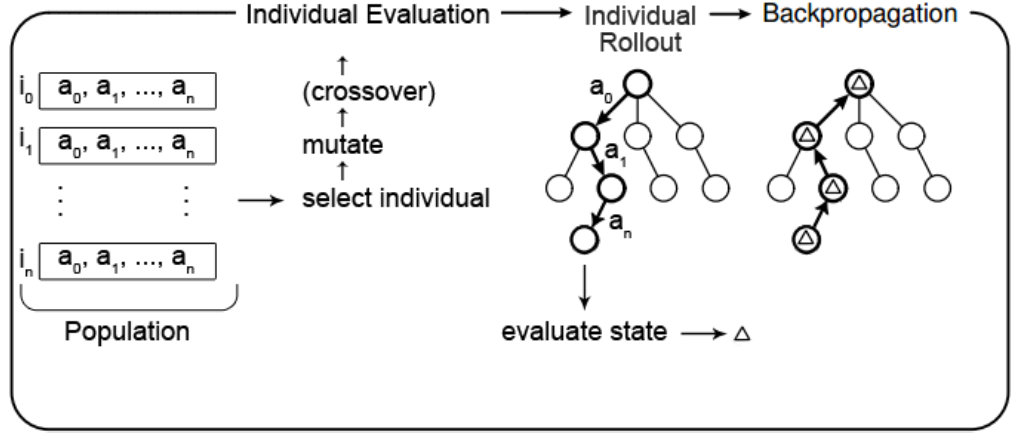
\includegraphics[width=0.5\textwidth]{RHEArollout}
		    		 \caption{RHEA statistical tree steps. Image sourced from \cite{gaina2017rolling}. }
		  		 \label{fig:RHEArollout}
			\end{figure}
			
			% Stages of Evilutionary algorithms
			
			
			A Typical genetic algorithm is composed of several stages;
			First the algorithm creates a population of random individuals, then it will iteratively go though the sample and calculate the fitness (i.e. the evaluation function as described in \ref{sssec:Common}) of every individual in the population. 
			The most fit individuals are then used to form a new generation, and each individual is modified with a combination of crossover and mutation. 
			Crossover is representative of biological reproduction where a child is produced based of the parents properties. Mutation is where a random value is changed to explore the search space and is analogous to biological mutation \cite{back1996evolutionary, vcrepinvsek2013exploration, perez2013rolling, gaina2017rolling, gaina2017analysis}.
			This process can be shown in figure \ref{fig:RHEArollout}.
			


			%Combination of RHEA AND MCTS
			Recent literature on AGI have been combining evolution and tree search in interesting ways in order to combine the benefits of both methods, such as Lucas et al. \cite{lucas2014fast} applied an EA process to guide the simulation step of MCTS and improve the random default policy. Their results show a significant increase in performance in the game \textit{Space Invaders} and the Mountain Car Problem.
			
		
		
		\subsubsection{Minimax}

				Minimax attempts to minimize the opponent's maximum reward at each state. The tree search is often stopped prematurely and a value function is used to estimate the outcome of the game, then the Alpha-Beta heuristic is used to prune the search tree \cite{browne2012survey, knuth1975analysis}.
			
		\subsubsection{Depth First Search}
				Depth First Search (DFS) is a tree search algorithm that iteratively expands each unvisited child node of the tree until a non-expandable node is reached. The search then navigates back up the tree until it finds the next unvisited node to expand and continues the search until all the nodes have been visited \cite{perez2014solving}.
				Depth first search with alpha-beta pruning \cite{knuth1975analysis} has achieved superhuman performance in chess, checkers and orthello. However it has not been effective in the game Go \cite{silver2016mastering}.
			
		
		
		\subsubsection{Breadth First Search (BFS) }\label{sssec:BFS}
			This paper proposes an efficient implementation of BFS for GVGP \cite{EfficientBFS} which uses a hash function.

	\subsection{Hyper-Heuristics}
		A hyper-heuristic approach typically combines several AI methods and automate them to be able to choose the best solution for that situation, a term used to describe them is `\textit{heuristics to choose heuristics}' \cite{burke2013hyper, burke2010classification}.
		During the 2015 competition, the three winning controllers all were a type of hyper-heuristic \cite{horn2016mcts}.
		
		

			
		
		

	\subsection{The General Video Game AI Competition} \label{ssec:GVGAIC}
	
		%General Video Game AI
		In most modern video games the AI is tailored specifically for that game and can't easily be modified for use in a different game type. However this is what GVG-AI aims to solve, by creating an AI that can play any game. 
		
		There have been quite a few AI competitions before in video games, such as Unreal Tournament \cite{hingston2010new}, Super Mario Bros \cite{shaker2013turing}, Starcraft \cite{ontanon2013survey}. 
		However most of the winning AI strategies used in those games are very domain specific and it is often more about knowing the game than developing good general AI \cite{perez20162014}. 
		 \par
		
		
		%GGP
		Another competition that was similar to GVG-AI was the General Game Playing (GGP) competition \cite{GGP2005general, love2008general}. However almost all of the games in the GGP are board games, and the Game Description Language (GDL) used is not designed for video games.
		
		%GVGAI Competiton
		The GVG-AI Competition is a competition framework that proposes the challenge of creating controllers for general video game playing. The controllers must be able to play a wide variety of video games, many of them will be completely unknown to the controller. This means the controller must have some general AI to discover the mechanics and goal of the game, so it can increase its score and win the game. \cite{GVGAI, perez20162014}
		
		The framework contains a library of 2D video games some of which are based of classic arcade games, there are currently as of writing this, 82 different singleplayer games and 20 multiplayer games that AI controllers can be tested on.
		
		%VGDL
		Games in the GVG-AI competition are written using the Video Game Description Language \cite{schaul2014extensible}, which is a high level description language designed to be able to create a wide variety of arcade style games, where the rules take the form of sprite movement and interaction on a 2D grid \cite{nelson2016investigating}.
		VGDL in GVG-AI is a JAVA port from pyVGDL which was programmed in python. The VGDL is a powerful tool for conducting research on computational intelligence and games \cite{schaul2014extensible, love2008general}.

		%ALE
		The Arcade Learning Environment \cite{bellemare2013arcade} provides an interface to hundreds of Atari 2600 game environments. ALE is similar to GVG-AI in a couple of ways; firstly it provides a test bed for benchmarking AI techniques within video games and secondly it is focused around creating agents within video games, as opposed to the GGP competition \cite{GGP2005general}.
		The Atari 2600 is a video game console developed in 1977 , it has had over 500 original games released for the console, and nearly all popular arcade games at the time were pored to the console such as; \textit{PAC-MAN} and \textit{SPACE INVADERS} \cite{bellemare2013arcade}. This provides a large test-bed for AI agents.
		The hardware for the Atari 2600 is very limited compared to today's standards, it had a 1.19Mhz CPU and 128 Bytes of RAM. These hardware specifications limit the complexity of the games that can be played on it, which strikes a balance of challenging but allowing search algorithms to have a small enough search space as to not have a large horizon effect \cite{bellemare2013arcade}.
		ALE has been used deep reinforcement learning techniques, that have been able to reach human level of play \cite{mnih2015human, gaina2017rolling}.
		

		
		
		
		%Summary
		The growing interest in competitions such as the ones mentioned above clearly reflects a desire for general competency for AI within games.

	\subsubsection{Challenges and Goals of GVG-AI}

		The goal of GVG-AI is to create a generally intelligent agent that is able to win any game it is placed in, when it doesn't know the game.
		During the tournament a completely new set of games are used, to avoid the agents becoming too domain specific.
		Another challenge is the time limit that an agent can choose an action, this avoids the agent spending too long deciding a task and not making an action \cite{schuster2015mcts}. 
		Furthermore this also is what defines the difference between GVG-AI and GGP, because having such a short amount of time to compute an action is what makes the competition such a challenge, otherwise the agent will be able to brute force the search space to find the best possible solution, which may take minutes or hours to compute each game tick.
		
		
	\subsubsection{Competition \& Rules}
	
		The winning conditions are decided by three factors:
		\begin{itemize}
		    \item Number of games finished with a victory
		    \item Total sum of points
		    \item Total time spent
		\end{itemize}
		The fist objective to be considered is the number of victories, however in case of a tie, the next objective is the number of points. Then if those two are a tie then the final decider is the total time spent before the win \cite{perez20162014}.
		In the competition the agent will play 10 unknown games and 5 levels per game. Furthermore each level is played ten times, so each agent plays roughly 500 total games in the tournament \cite{schuster2015mcts}.
		The competition does now allow multithreading that is used by some MCTS enhancements, some MCTS enhancements that are used are discussed in section \ref{sssec:MCTSvariations}.
		The controllers can also use up to 1 second of CPU time for initialization and 40ms to compute an action each game tick. However if the controller takes between 40ms and 50ms, the action return will be \textit{NIL}(Where no movement will be applied), anymore than 50ms will result in the controller automatically loosing \cite{horn2016mcts, perez20162014}.
	
	
	\subsubsection{The GVG-AI Framework \& Sample Controllers} \label{Framework}
	
		%Limits of the framework
		The Framework is developed in the Java Environment and has a few differnet tracks that you can submit AI for, these are; Single Player Planning Track, 2-Player Planning Track and Level Generation Track \cite{gaina2016general}.
		The controllers are allowed upto 40ms to compute the agents action(s) \cite{perez2016GVGAICompetition, GVGAI}.
		
		
		These sample agents provide useful insights into how new agents can be created for the competition by applying common AI techniques.
		The \textit{HUMAN} player and the \textit{REPLAYER} can be used for debugging the game and to help the programmer get a better understanding of how the game can be played.
		
		
		The framework uses a Video Game Description Language (VGDL) to describe a wide variety of video games. The VGDL is based on a python version developed by Schaul (2014) called PyVGDL \cite{schuster2015mcts}. Furthermore in the GVG-AI Competition the AI agent does not have access to the whole games description, where as in GGP the agent was able to see the whole game description. This means that the agent has to analyze and simulate the game in order to figure out the rules and goal of the game.
		
		
		The framework has an StateObservation object that has an interaction set that consists of \textit{up, down, left, right, nil, escape} and \textit{use}.

		The GVG-AI framework comes with quite a few sample agents;
		
		\textbf{Sample MCTS} \label{sssec:sampleMCTS}
			The GVG-AI framework proves a sample MCTS controller, this controller has received considerable interest due to its success in the competition. 
			The sample MCTS controller is an implementation of the vanilla MCTS algorithm, this is described in section \ref{sssec:MCTS}, and the full description of MCTS algorithm is described by Browne et al. \cite{browne2012survey}.
			The sample MCTS controller uses a payout depth of 10 moves and an exploration-exploitation constant value of $\sqrt{2}$ (from equation \ref{eqUCT}) and selects the most visited action from the root to pick a move to return for each game cycle \cite{perez20162014}.
			However MCTS isn't the sole answer to the GVG-AI competition, as it has been shown that even with a 30x computational budget, it fails to master games. However it does manage to avoid to explicitly loosing games, but does not win a lot of them either. This shows that for the AI it finds not losing is significantly easier than winning \cite{nelson2016investigating}.

		\textbf{sample GA} \label{sssec:sampleGA}
			The sample Genetic Algorithm(GA) controller is a rolling horizon open loop implementation for a minimalistic steady state genetic algorithm, known as microbial GA \cite{harvey2009microbial, perez20162014}.
			A tournament takes place between two players and the loser of the tournament is mutated randomly, with the probability of 1/7. Then certain parts of its genome are recombined with parts from the winners genome, with the probability of 0.1 \cite{perez20162014}. 
			This repeats until the time budget has been used. The evaluation function is the same as the sampleMCTS controller. 
			The sample GA controller came 12th in the competition \cite{perez20162014}.
			

		\textbf{Random}
			This is a very simple controller that is provided with the GVG-AI framework, it simply returns a random action at each game cycle.
			The random controller came 14th in the competition, which is quite surprising as it managed to beat quite a few of the other, more complicated controllers \footnote{The reason for this may be due to more complicated controllers not choosing an action because it isn't able to search enough of the game space, so making a random action is often better than no action.}.

		\textbf{OSLA}
			One Step Look Ahead is another rather simple controller, it evaluates the position using the same heuristic as Sample MCTS and selects the action with the highest evaluation score, then moves the model one step ahead. This controller came in 16th place zcite{perez20162014}.

	
		
	
\section{Research Methodologies}	
	The data of the GVG-AI sample controllers as well as the controllers submitted for the competitions in previous years will be gathered. 

	% What data will be collected:
	These are a few of the type of metrics that will be gathered from the controllers:
	\begin{itemize}
		\item Success rate in a particular game.
		\item Where the agent was when it lost or won the game
		\item How much of the search space was the controller able to search
		\item The amount of moves that controller made in each type of game
	\end{itemize}

	%What I will create
	There will be thousands of different simulations to run to gather the required data, this will be done by modifications to the GVG-AI framework to gather the extra information needed.
	From this data this paper will aim to create an AI controller that will either use hyper-heuristics to improve its performance. Furthermore conclusions can be drawn out as to the limitations of different search techniques and potentially any areas in which they could be improved.
	
	

	%Justification of research
	This software will provide an in depth insight into the challenges faced by each tree search algorithm.
	Further research could include feeding this data back into the search algorithms or level generators to develop levels that the search techniques will be able to navigate.

	
\subsection{Hypothesis}
	\textbf{Null Hypothesis:}
		The different search trees methods have no significant differences in strength in the competition.
		
	\textbf{Hypothesis:}
		Combining different search techniques with different strengths and weaknesses lead to a better AI agent.

\section{Conclusion}
	In conclusion, the literature covered in this review provides an overview of a few of the current algorithms in use in the GVG-AI competition.
	Based on the performance of the different search algorithms within the framework, a conclusion will be drawn between the superior algorithms for certain games.
	The GVG-AI competition provides a good framework to compare different tree search algorithms. 
	The aim of this paper will be to create an agent for the GVG-AI competition based of the strengths and limitations of tree search algorithms.







%%%%%%%%%%% Requirements analysis and specification %%%%%%%%%%%%%%%%%%%%%%%

\section{Experemental Setup}

	% Choosing what games to test the tree search algorithms on
	\subsection{Choosing the Games}
	
	There are hundreds of games within the GVG-AI framework, and most have multiple levels, so testing with all the different possible configurations is prohibitively expensive, thus a subset of games within the framework will be selected in a way that will best represent the framework as a whole.
	
	%Other authors that have chosen the best games tio test
	There are papers by previous authors that looked into finding a good selection of games that can be used for benchmarking the framework. \cite{gaina2017population}
	
	In Mark Nelsons paper \cite{nelson2016investigating}, he presented a large scale analysis of MCTS with 62 games in the framework, which were sorted based on performance. Bontrager et al. \cite{bontrager2016matching} used clustering techniques on 49 games in the goal to obtain rough groups of similar games.
	The final 20 games that will be used in this paper are based of the paper by Gaina et al. \cite{gaina2017population} where they uniformly sampled from both Mark Nelson and Bontrager et al. papers and balanced a set of 10 stochastic and 10 deterministic games, which can be shown in figure \ref{GamesTable}.
	
	
	% Table of games
	\begin{table}[h!]
	\centering
	\begin{tabular} { |c||c|} 
		 \hline
		 \bf{Deterministic Games} & \bf{Stochastic Games} \\
		 \hline
		 Bait & Aliens  \\
		 \hline
 		Chase  & Chopper   \\
		\hline
		Hungry Birds  & Digdug   \\
		\hline
		Missile Command  & Intersection   \\
		\hline
		Plaque Attack  & Seaquest   \\
		\hline
		Camel Race  & Butterflies   \\
		\hline
		Escape  & Crossfire   \\
		\hline
		Lemmings  & Infection   \\
		\hline
		Modality  & Roguelike   \\
		\hline
		Wait For Breakfast  & Survive Zombies   \\
		\hline

	\end{tabular}
	\caption{Table of games selected based of \cite{guerrero2017beyond, gaina2017population}.}
	\label{GamesTable}
	\end{table}
	

%%%%%%%%%%% Design of research artifact %%%%%%%%%%%%%%%%%%%%%%%


%%%%%%%%%%% Implementation %%%%%%%%%%%%%%%%%%%%%%%


%%%%%%%%%%% Research Methodology %%%%%%%%%%%%%%%%%%%%%%%


%%%%%%%%%%% Method of evaluation the research artifact (Unit Testing) and findings %%%%%%%%%%%%%%%%%%%%%%%


%%%%%%%%%%% Professional Considerations %%%%%%%%%%%%%%%%%%%%%%%


%%%%%%%%%%% Conclusion %%%%%%%%%%%%%%%%%%%%%%%


%%%%%%%%%%% Acknowledgements %%%%%%%%%%%%%%%%%%%%%%%


	
\section{Research}
	\textbf{Preliminary results}
		By gathering data on the sampleMCTS controller, this heatmap of where the agent was 


	 

% references section

\bibliographystyle{IEEEtran}
\bibliography{references}

% Appendices

%\appendices
%\section{First appendix}
%Appendices are optional. Delete or comment out this part if you do not need them.

% that's all folks
\end{document}
